\newpage
\appendix
\renewcommand{\thechapter}{\Asbuk{chapter}}
\chapter{Описание приложения моделирования манипулятора} 
\section{Отличительные особенности} \label{app1start}

Данная программа является отдельным кроссплатформенным приложением, имеющим графический интерфейс. Приложение написано на языке высокого уровня Java. Для построения графического интерфейса был использован фреймворк JavaFX.

Особенности приложения:
\begin{itemize}
\item{Возможность ввода пользователем собственного закона управления для манипулятора в аналитическом виде. Причем, при вводе допускаются как использование элементарных функций, так и инегралов, в том числе, приводящих к уравенениям с запаздыванием (пределы интегрирования зависят от времени)}
\end{itemize}

Все изображения, используемые в приложении защищены авторским правом, алгоритмы и методы, используемые в приложении являются интеллектуальной собственностью автора.  . Патент РФ на программу для ЭВМ №.  Москва, Роспатент, заявка № . Дата поступления .  Дата государственной регистрации в Реестре программ для ЭВМ . 

Приложение служит для моделирования движения управляемого трехзвенного манипулятора, анализа управления, времени стабилизации движения манипулятора относительно заданного положения или траектории. Результаты моделирования используются в главах 2 и 3 настоящей диссертации.

Для запуска приложения вне зависимости от операционной системы, на которой оно исполняется, необходимо запустить файл manipulator.jar. На стартовом экране пользователь может выбрать переход к теоретической части, в которой описана математическая модель и алгоритмы, лежащие в основе работы программы либо перейти непосредственно к разделу моделирования.

\begin{figure}[h]
\center{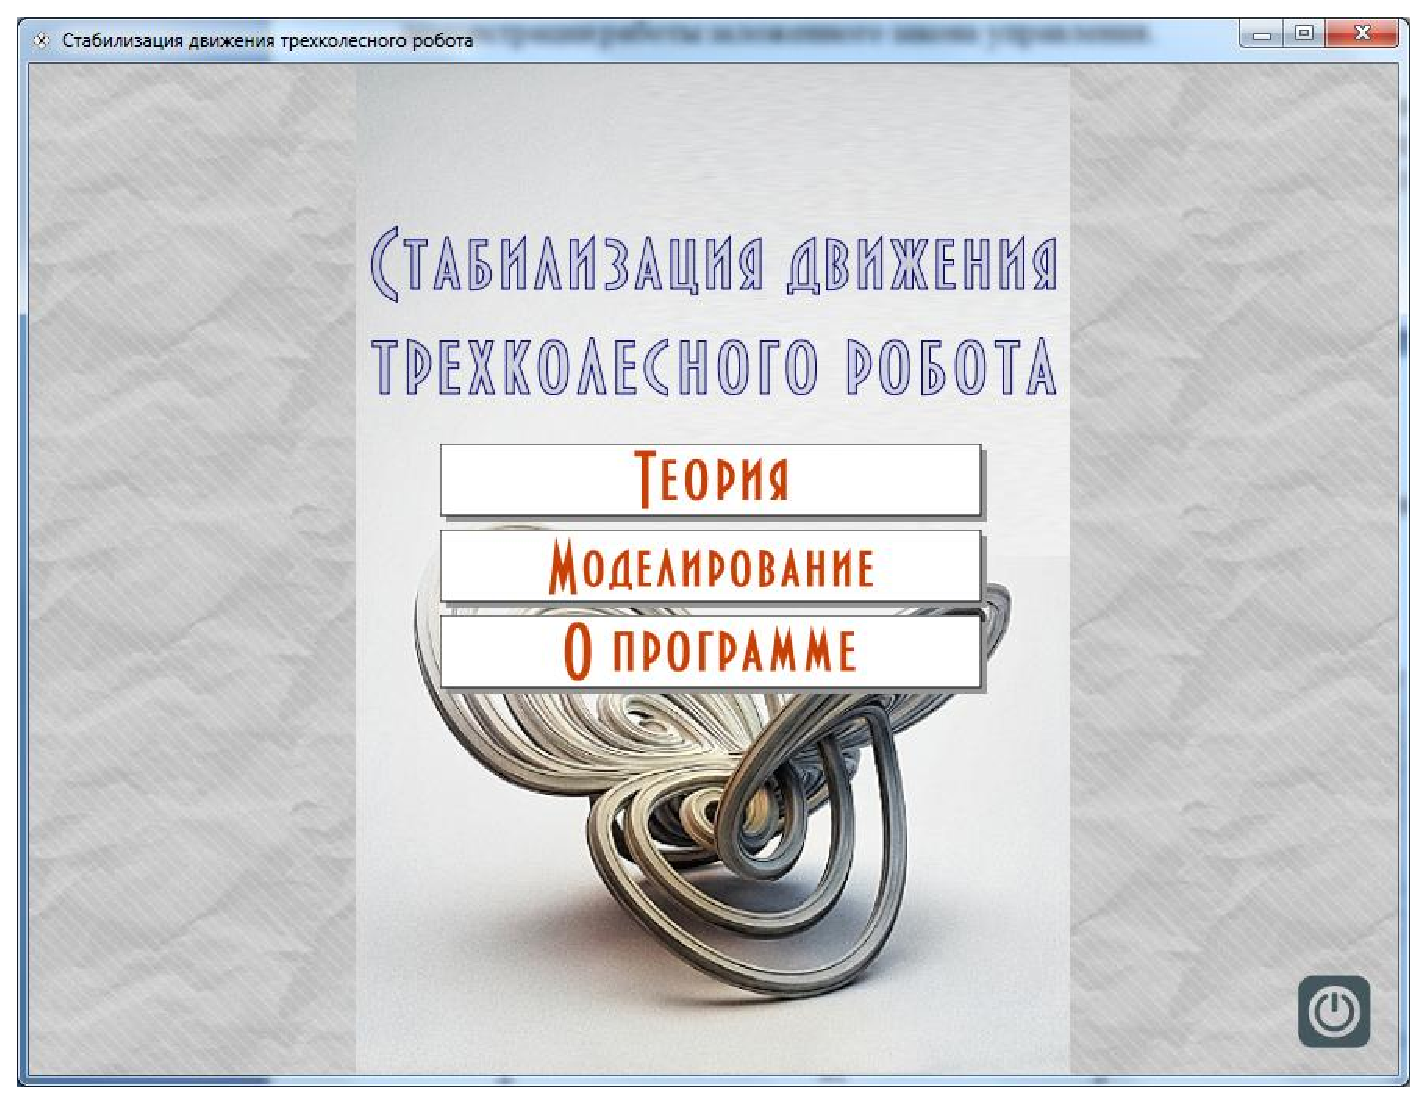
\includegraphics[width=1\linewidth]{window}}
\caption{Основной экран программы}
\label{ris:window}
\end{figure}

\par
\textbf{Теоретический раздел}

В теоретическом разделе содержится схематическое изображение манипулятора, система дифференциальных уравнений, описывающих его движение и краткое теоритеское основание построения управления манипулятором. Подробные теоретические выкладки содержатся в главе 3 настоящей  диссертации.
\nopagebreak[4]
\begin{figure}[h]
\center{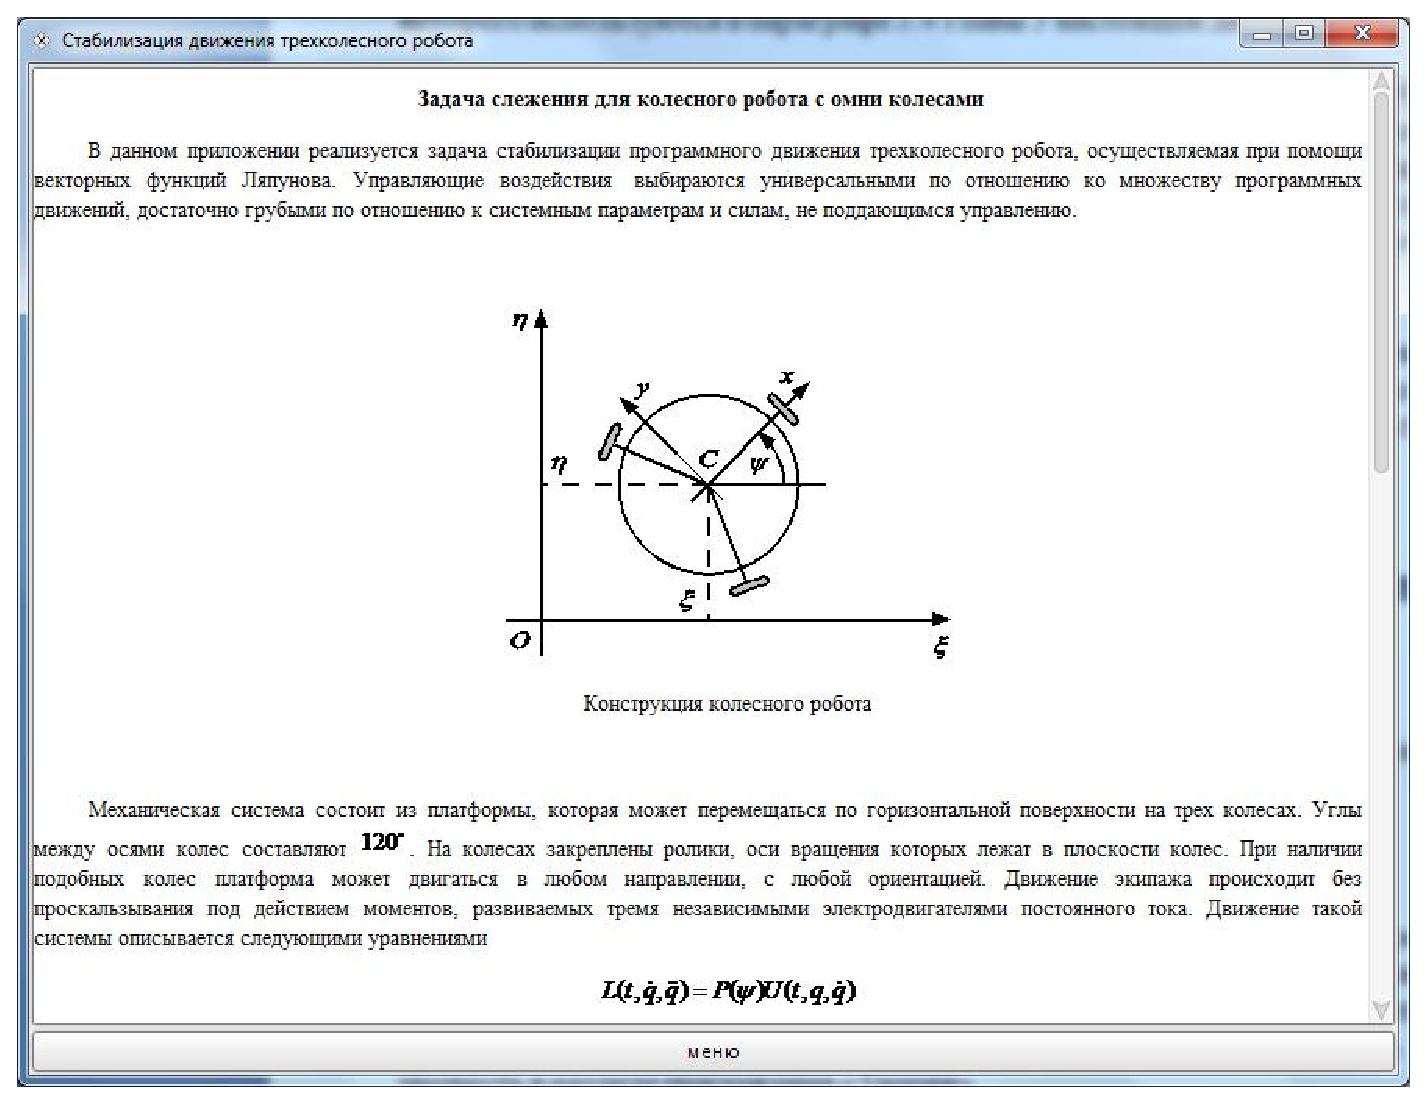
\includegraphics[width=1\linewidth]{theory}}
\caption{Внешний вид теоретического раздела}
\label{ris:theory}
\end{figure} 

\par
\textbf{Раздел моделирование}

В разделе непосредственного моделирования пользователю предлагается задать параметры системы, такие как геометрические характеристики манипулятора (длины звеньев, расстояния до их центров масс), массы звеньев, начальные положения звеньев, а также законы управления в аналитическом виде. Также присутствует возможность автоматического заполенения заранее подобранными значениями по умолчанию для демонстрации работы программы. Значение каждого параметра представлено в теоретическом разделе, на экране моделирования же присутсвуют только сокращенные обозначения, совпадающие с обозначениями в теоретической части.

\begin{figure}[h]
\center{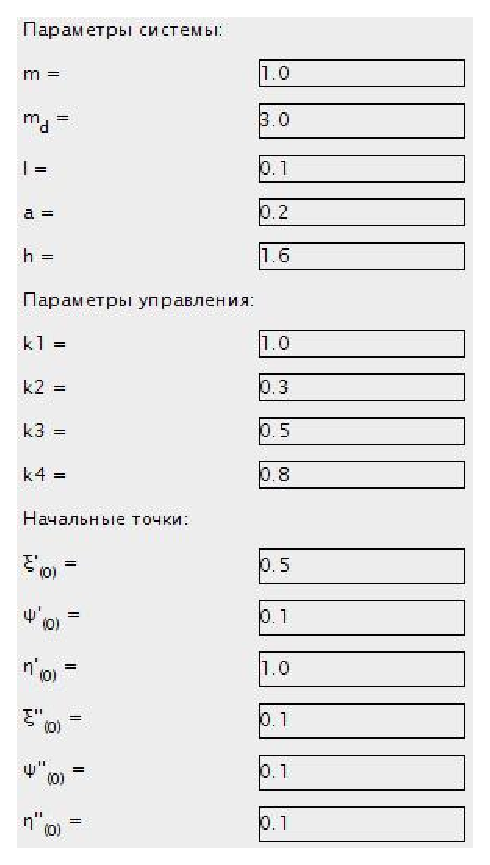
\includegraphics[width=0.5\linewidth]{params}}
\caption{Параметры для расчетов}
\label{ris:params}
\end{figure} 

\begin{figure}[h]
\center{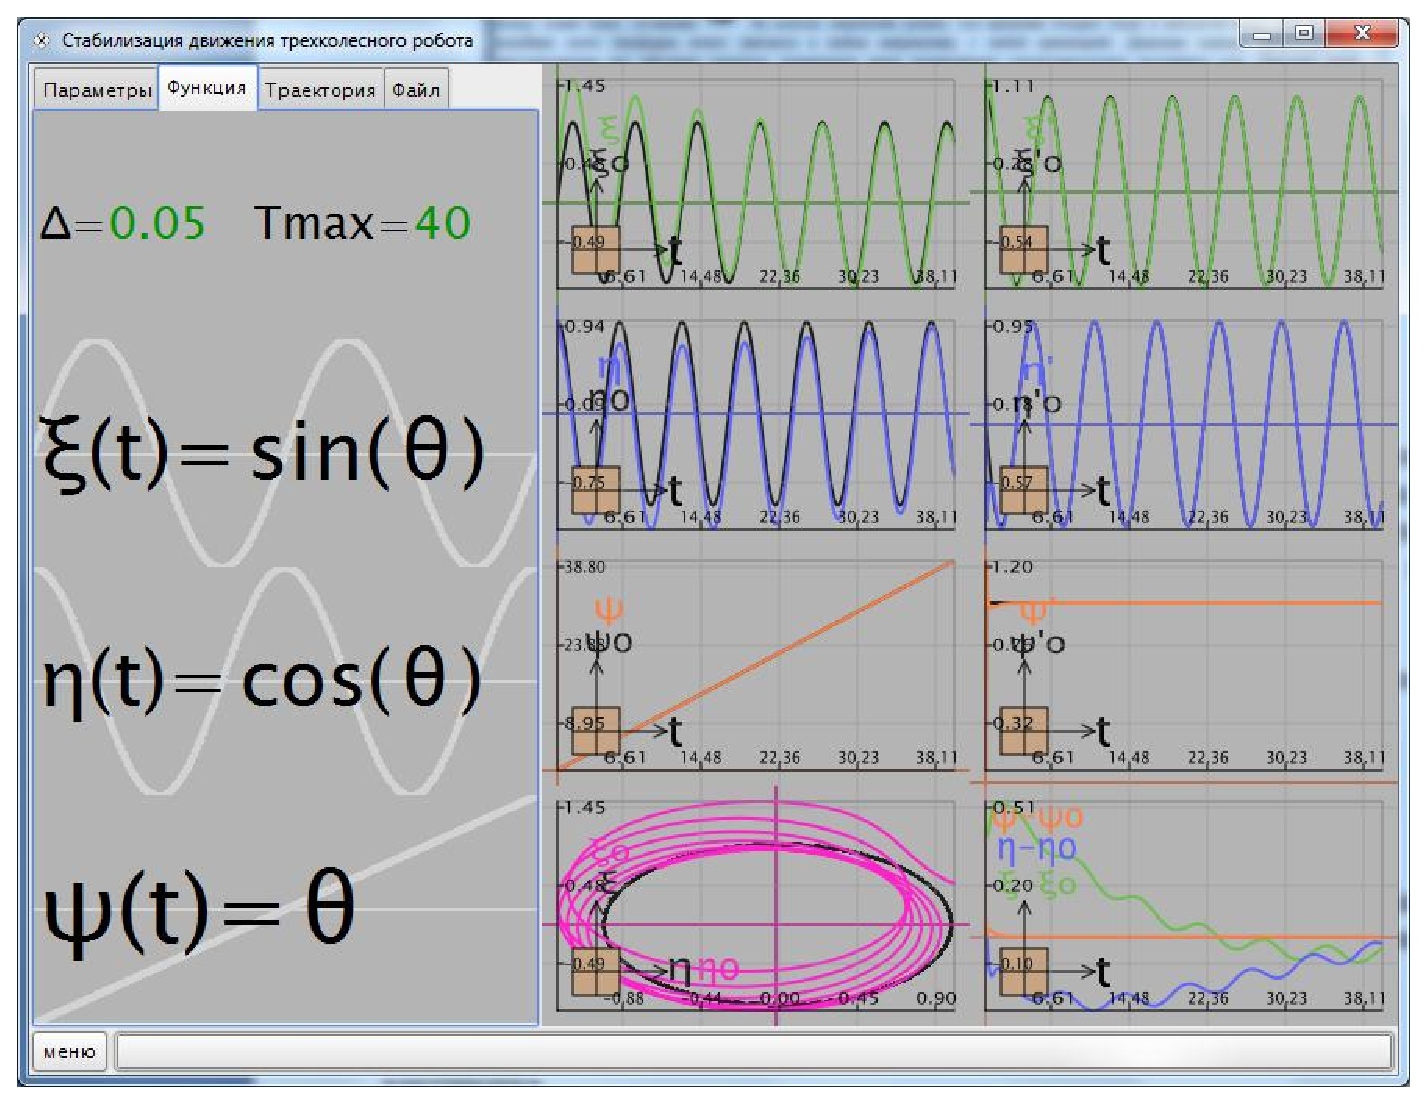
\includegraphics[width=1\linewidth]{modeling}}
\caption{Внешний вид раздела моделирование}
\label{ris:modeling}
\end{figure}

В случае возникновения ошибки, программа сообщает о ней, выделяет незаполненные поля в случае недостаточных данных.
\par
\textbf{Задание закона управления манипулятором аналитически}

Для обработки введенных формул используется открытая сторонняя библиотека, позволяющая пользователю вводить элементарные функции. Также библиотека была доработана для того, чтобы иметь возможность распознавать определенные интегралы с переменным верхним или нижним пределом.

Формулы вводятся в поля ввода в качестве строк текста. В формулах допускается использование констант, основных математических операций и параметров системы, таких, например, как массы звеньев, заданные в виде переменных. При обработке формул происходит преобразование текста в объекты языка Java и сохранение в оперативной памяти. Дальнейшие вычисления проводятся с помощью подстановки вместо переменых констант, необходимых для работы на текущем шаге. Таким образом, обработка формулы производится только на первых шагах, что положительно сказывается на скорости работы программы.

При необходимости библиотке работы с формулами может быть расширена.

Первоначально пользователю предлагается дискретизации $\delta$  и время моделирования  $T_{max}$ рис.\eqref{ris:formul}. После ввода ввода уравнений управления и параметров системы пользователь нажимает на кнопку построения графиков, после чего программа производит моделирование движения манипулятора и отображает результаты в виде графиков, показывающих соответствующее изменение координат каждого из звеньев, а также изменения скоростей звеньев с течением времени, ограничиваясь максимальным временем, заданным пользователем.

\begin{figure}[h]
\center{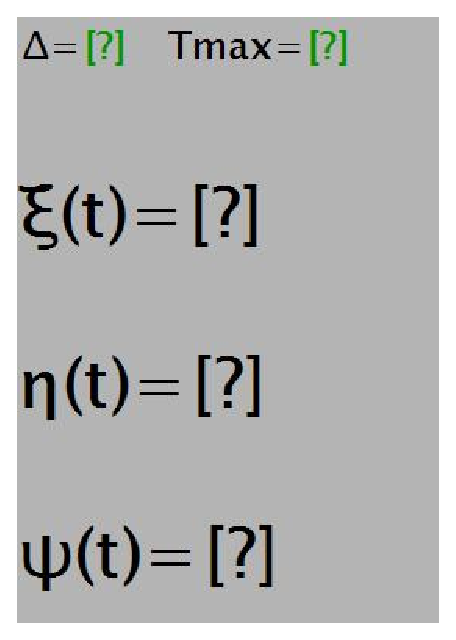
\includegraphics[width=0.5\linewidth]{formul}}
\caption{Система ожидает ввода управления с помощью формул}
\label{ris:formul}
\end{figure}

При наборе формулы поддерживаются следующие действия:
\begin{itemize}
\item{основные математические операции (сложение, вычитание, умножения, деление, возведение в степень);}
\item{ввод формул без ограничения на длину;}
\item{ввод без ограничений по количеству вложенных скобок;}
\item{добавление делегированных тригонометрических и алгебраических функций ($sin(t), cos(t), tg(t), ctg(t), exp(t), ln(t)$ );}
\item{ввод определенных интегралов в том числе с подынтегральной функцией и пределов интегрирования в зависимости от времени $t$;}
\item{ввод независимой переменной $t$;}
\end{itemize}

\textbf{Ввод данных из файла}

При этом вводе данных пользователю необходимо выбрать файл, содержащий заданное управление и параметры системы. В данный момент программой поддерживается два формата хранения данных

\begin{itemize}
\item{cvs;}
\item{json}
\end{itemize}

\begin{figure}[h]
\center{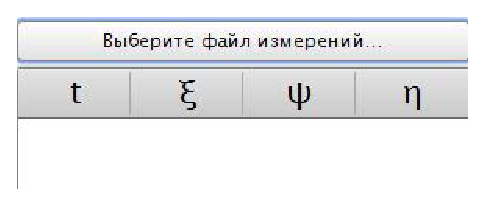
\includegraphics[width=0.5\linewidth]{mass}}
\caption{Внешний вид формы для ввода массива данных}
\label{ris:mass}
\end{figure}

Очередность параметров, считываемых из файла соответсвует порядку их расположения на графическом интерфейсы работы с программой. Так сначала идут параметры системы, затем начальные координаты и скорости звеньев, затем законы управления движением звеньев.

В качества разделителя данных используется символ ";". Дробные числа записываются через символ ".".

\par
\textbf{Расчетная часть}

Для детального ознакомления с реализацией расчета см. Приложение 1.
После задания траектории движения робота одним из описанных способов, в правой части приложения выводятся следующие графики рис.\eqref{ris:graph}

\begin{enumerate}
\item{ графики  $\xi(t), \xi_0(t)$ траектории центра масс платформы }
\item{ графики  $\eta(t), \eta_0(t)$ координаты  центра масс платформы }
\item{ графики  $\psi(t), \psi_0(t)$ угла поворота платформы  }
\item{ графики  $\dot{\xi(t)}, \dot{\xi_0(t)}$ скорости центра масс платформы }
\item{ графики  $\dot{\eta(t)}, \dot{\eta_0(t)}$ скорости координаты  центра масс платформы }
\item{ графики  $\dot{\psi(t)}, \dot{\psi_0(t)}$ скорости поворота платформы  }
\item{ графики траектории платформы  на фазовой плоскости $\xi(\eta(t)), \xi_0(\eta_0(t))$}
\item{ графики  $\|\dot{\xi(t)} - \dot{\xi_0(t)}\|$, $\|\dot{\eta(t)} - \dot{\eta_0(t})\|$, 
$\|\dot{\psi(t)} - \dot{\psi_0(t)}\|$  }
\end{enumerate}
При построении графиков  использовался пятиточечный метод численного дифференцирования.

По графикам можно судить, что рассматриваемая система двигается вдоль отслеживаемой траектории на расстоянии, не превышающем погрешности слежения.

\begin{figure}[h]
\center{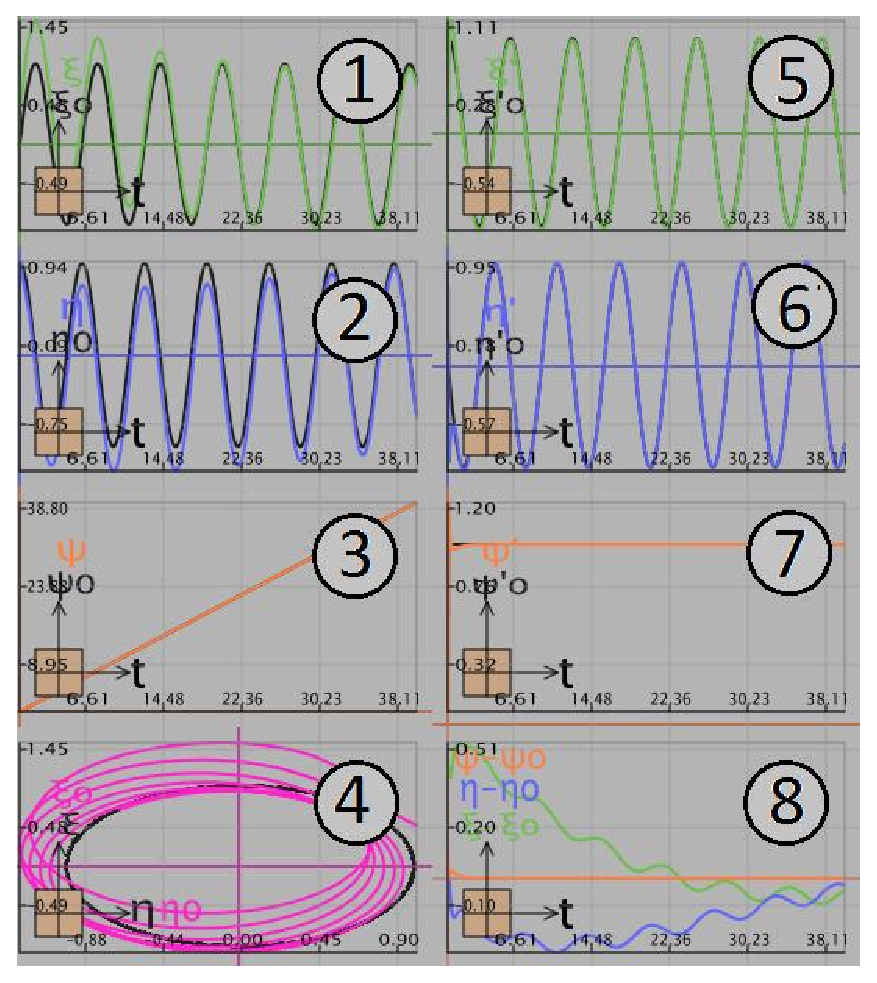
\includegraphics[width=1\linewidth]{graph}}
\caption{Внешний вид расчетной части}
\label{ris:graph}
\end{figure}


